%%%%%%%%%%%%%%%%%%%%%%%%%%%%%%%%%%%%%%%%%
% University/School Laboratory Report
% LaTeX Template
% Version 3.1 (25/3/14)
%
% This template has been downloaded from:
% http://www.LaTeXTemplates.com
%
% Original author:
% Linux and Unix Users Group at Virginia Tech Wiki 
% (https://vtluug.org/wiki/Example_LaTeX_chem_lab_report)
%
% License:
% CC BY-NC-SA 3.0 (http://creativecommons.org/licenses/by-nc-sa/3.0/)
%
%%%%%%%%%%%%%%%%%%%%%%%%%%%%%%%%%%%%%%%%%

%----------------------------------------------------------------------------------------
%	PACKAGES AND DOCUMENT CONFIGURATIONS
%----------------------------------------------------------------------------------------

\documentclass{article}

\usepackage{graphicx} % Required for the inclusion of images
\usepackage{amsmath}
\usepackage{float}
\usepackage{indentfirst}
\usepackage[margin=1in]{geometry}
\usepackage[framed,numbered]{matlab-prettifier}
\usepackage{array}
\usepackage{amssymb}
\usepackage{caption}
\usepackage{multirow}
\setlength{\parskip}{\baselineskip}
\renewcommand{\labelenumi}{\alph{enumi}.} 
\setlength\extrarowheight{2pt}
\usepackage{times}
\usepackage{color} %red, green, blue, yellow, cyan, magenta, black, white
\definecolor{mygreen}{RGB}{28,172,0} % color values Red, Green, Blue
\definecolor{mylilas}{RGB}{170,55,241}

%----------------------------------------------------------------------------------------
%	DOCUMENT INFORMATION
%----------------------------------------------------------------------------------------

\begin{document}

\begin{center}
\begin{tabular}{l}

\textbf{Functionality Outline}\\
\\
Simulation of Mendelian Laws of Genetics\\
\textbf{Programming Assignment} 2\\
\\

Date: March 30th, 2018\\
\\
\textbf{Prepared by}\\
Sean Mitchell\\
sm0077@uah.edu\\
\\

\textbf{Prepared for}\\
Dr. Rick Coleman\\
CS 307 - 01: Object Oriented Programming in C++\\
Computer Science Department\\
University of Alabama in Huntsville\\

\end{tabular}
\end{center}

%----------------------------------------------------------------------------------------
%	SECTION 1
%----------------------------------------------------------------------------------------
\newpage
\setcounter{tocdepth}{4}
\setcounter{secnumdepth}{4}
%\renewcommand*\contentsname{Table of Contents}
\tableofcontents
\newpage

\section{System Overview}
\hrule
\subsection{UML Diagram}
\begin{center}
\begin{minipage}{\textwidth}
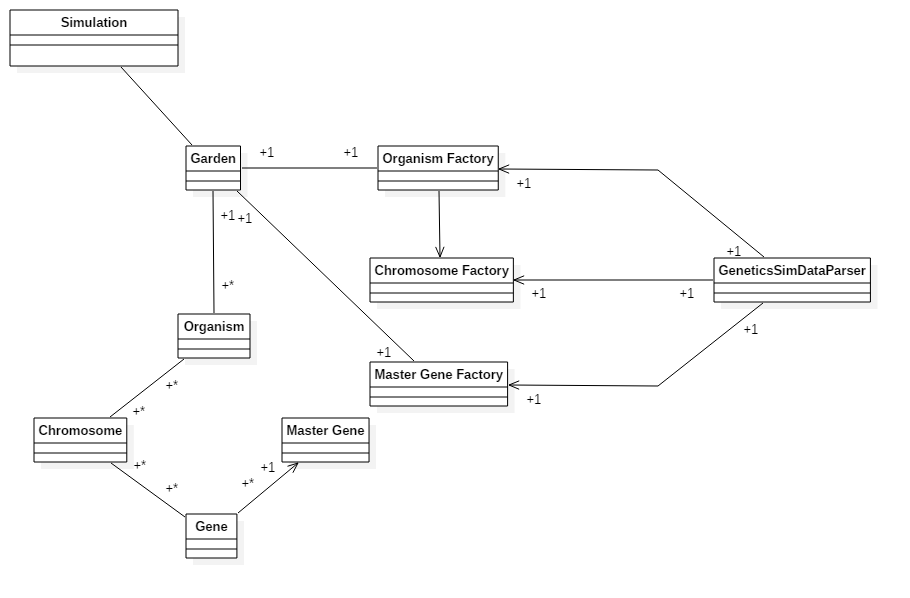
\includegraphics[width=1\linewidth]{Main.png}
\captionof{figure}{Preliminary UML Class Diagram}
\end{minipage}
\end{center}

\section{Class Descriptions}
\begin{description}

\item[Simulation] The Simulation class will perform three main tasks. The first task will be to ask the user how many offspring to create. The second task will be asking the user the name of the data file to read as input. Using the input from the first two tasks, the Simulation object will create an instance of Garden, passing the number of children to create and the input file as arguments.

\item[Garden] The Garden class will perform several tasks. The first task will use the data file passed as input to create two parent Organism objects. Once these two parents have been created, the Garden object will allocate data structures to store the children. Next, the Garden object will breed the two parents until the number of offspring created matches the input received from the Simulation object. Once all the offspring are created, the Garden object will sort the data structures. Finally the Garden object will return a report of the results of the simulation.

\item[Parser] The Parser object will read the attributes of each gene. This object will be called by the factories to return the data needed to for the factories to create their instances.

\item[Organism] The Organism class will be an instance of the object returned from the Organism Factory. The class will contain a Chromosome vector which will store all the Chromosome objects that the Organism has. Other member variables that class will have include both the common name and scientific name. The class will also have accessor and mutator functions to these member variables.

\item[Organism Factory]The Organism Factory will perform the creation of instances of Organism. The Organism Factory class is a simple factory. The Organism Factory shall use the Chromosome Factory to create chromosomes for organisms. The Organism Factory shall contain a function which returns an instance of an organism with fully defined genotype. This factory will also be a Singleton.

\item[Chromosome] The Chromosome class will be an instance of the object returned from the Chromosome Factory. Instances of Chromosome will store the genes for that particular chromosome. 

\item[Chromosome Factory] The Chromosome Factory class will perform the creation of instances of chromosomes. This class will be a simple factory. The Chromosome Factory shall use the Master Gene Factory to create genes for chromosomes. This factory will also be a Singleton.

\item[Gene] The Gene class will be an instance of the object returned from the Gene Factory. The Gene class will hold a reference to the master gene and variables to hold the specific allele characters for that instance of the gene.

\item[Master Gene] The Master Gene class is a single instance for each type of gene. This instance will hold most of the information that is common to many genes.

\item[Master Gene Factory] The Master Gene Factory class will perform the creation of instances of both Master Gene and Gene. This class is a simple factory. This factory will also be a Singleton.

\end{description}

\section{Background Infomation}
\hrule
In 1866 an Austrian monk named Gregor Mendel published a paper in Proceedings of the Natural Society of Brunn, in which he described the laws of genetics which he had formulated from his work cultivating, cross-breeding, and testing thousands of pea plants (Pisum sativum). Some of the traits he studied were plant stature (tall vs. dwarf), seed color (green vs. yellow), and seed pod texture (smooth vs. wrinkled). While getting little attention from the scientific community at first, his work later became the foundation for the entire science of genetics and today Mendel is known as the "father of modern genetics."

Mendel showed that for any particular trait, such as plant stature, there were actually two genes forming a matched gene pair to determine the trait. Each of the genes in the pair could be either of two types. One gene type produced tall plants. This he represented with a T. The other produced dwarf plants and he represented this with a t. Thus, to represent the genotype or genetic makeup of a plant with regard to stature he could use, TT, Tt, or tt. He found that if a plant had at least one "tall" gene (represented as TT or Tt) it was always tall. This gene type he called dominant. Only when the genotype for a plant’s stature was represented as tt was it a dwarf plant. This gene type he called recessive. 

Mendel came to this conclusion when he found that if he crossed a plant that always produced tall offspring, i.e. was pure-bred tall, with a plant that always produced dwarf offspring, i.e. was pure-bred dwarf, he got not medium sized plants but all tall plants. And, when he crossed these plants he got both tall and dwarf plants in a ratio of three tall to one dwarf. Mendel said that organisms have genes for traits in pairs. That when reproducing each parent plant contributes one of their pair of genes for each trait to each of the offspring. Which gene of the pair is contributed is purely random. This is easy to see if we look at a diagram representing the possible combinations. On the left we see the possible combinations when crossing a pure-bred tall (also called homozygous tall) with a pure-bred dwarf (also called homozygous dwarf) plant. All the offspring will be hybrid tall (also called heterozygous tall). When two of these hybrid plants are crossed we see that the phenotypes (visible traits) give a ratio of tall to dwarf plants of 3:1. The possible genotype combinations give a ratio of one homozygous tall to two heterozygous tall to one homozygous dwarf.



%----------------------------------------------------------------------------------------
%	SECTION 2
%----------------------------------------------------------------------------------------

\newpage
\section{Object Functionality}
\hrule
\subsection{CS\_307\_Main.cpp}
\subsubsection{Main()}
\indent Instantiate Simulation object\\
\indent Call Simulation$\rightarrow$Sim\_Main()\\

\subsection{Simulation.cpp}
\subsubsection{Simulation()}
\indent Declares member variables

\subsubsection{\textasciitilde Simulation()}
\indent Calls delete on all objects within the object

\subsubsection{Sim\_Main()}
\indent Ask for number of children as input\\
\indent Store received input in int variable \\
\indent Ask for name of input data file\\
\indent Store received input in string variable \\
\indent Instantiate Garden object\\
\indent Call Garden $\rightarrow$ Garden\_Main() \\
\indent Call Sim\_Report() \\

\subsubsection{Sim\_Report()}
\indent Queries the Garden object for the number of entries in its internal data structures\\
\indent Prints out the results of this query to the terminal\\

\newpage
\subsection{Class Garden}

\subsubsection{Garden()}
\indent Declares member variables\\
\indent Declares parent vector \\
\indent Declares child vector \\
\indent Declares report vector \\
\indent Declares detailed report vector \\
\indent Instantiate Organism Factory object\\
\indent Instantiate Chromosome Factory object\\
\indent Instantiate Master Gene Factory object\\
\indent Instantiate master objects\\
\indent Instantiate parent Organism objects\\
\indent Store parent Organism objects in parent vector\\

\subsubsection{\textasciitilde Garden()}
\indent Calls delete on all objects within the object

\subsubsection{Garden\_Main()}
\indent Instantiate parent\_1 object\\
\indent store parent\_1\\
\indent Instantiate parent\_2 object\\
\indent store parent\_2\\
\indent Call Breed()\\

\subsubsection{Breed()}
\indent Loop from 0 to number\_of\_children\\
\indent\indent pass parent objects to organism factory\\
\indent\indent Add that child from the organism factory to the children vector\\

\subsubsection{Get\_Child\_Vector()}
\indent Returns the child vector

\newpage

\subsection{Class Parser}
\subsubsection{GeneticsSimDataParser()}
\indent Declares member variables\\
\indent Instantiate parser objects\\

\subsubsection{\textasciitilde GeneticsSimDataParser()}
\indent Deletes parser objects\\

\subsubsection{getGeneCount()}
\indent Returns m\_iNumGenes\\

\subsubsection{getGenus()}
\indent Returns m\_sGenus\\

\subsubsection{getSpecies()}
\indent Returns m\_sSpecies\\

\subsubsection{getScientificName()}
\indent Returns m\_sSciName\\

\subsubsection{getCommonName()}
\indent Returns m\_sCommonName\\

\subsubsection{getGeneData()}
\indent Open input file\\
\indent Walk through file\\
\indent\indent Set next gene to member variables\\
\indent Close file\\

\subsubsection{getParentGenotype()}
\indent Open input file\\
\indent Walk through file\\
\indent\indent Get parent genotype
\indent Close file\\

\newpage

\subsection{Class Organism Factory}

\subsubsection{Organism\_Factory()}
\indent Private constructor

\subsubsection{Organism\_Factory Instance()}
\indent Returns the instance of the organism factory

\subsubsection{Breed(parent\_1, parent\_2)}
\indent Calls the chromosome factory object, passing the two parents as arguments
\indent Returns the new child organism

\newpage

\subsection{Class Organism}
\subsubsection{Organism()}
\indent Creates parent Organism object \\
\indent Calls chromosome factory, passing the chromosomes the child organism received as arguments \\
\indent Store chromosomes in the Organism's chromosome vector \\

\subsubsection{\textasciitilde Organism()}
\indent Calls delete on all objects within the object

\subsubsection{Set\_Name()}
\indent Sets the name field to the input of this function

\subsubsection{Get\_Name()}
\indent Returns the name field

\subsubsection{Set\_Attribute()}
\indent Sets the attribute field to the input of this function

\subsubsection{Get\_Attribute()}
\indent Returns the attribute field

\subsubsection{Set\_Gene()}
\indent Appends the input onto the gene vector

\subsubsection{Get\_Gene()}
\indent Returns the gene vector

\newpage

\subsection{Class Chromosome Factory}

\subsubsection{Chromosome\_Factory()}
\indent Private constructor

\subsubsection{Chromosome\_Factory Instance()}
\indent Returns the instance of the chromosome factory

\subsubsection{Breed(parent\_1\_chromosome, parent\_2\_chromosome)}
\indent Calls the master gene factory object, passing the two chromosomes as arguments\\
\indent Returns the new child chromosome vector\\

\newpage

\subsection{Class Chromosome }

\subsubsection{Chromosome()}
\indent create chromosome vector\\

\subsubsection{Get\_Chromosome()}
\indent Returns the chromosome vector

\newpage
\subsection{Class Gene}
\subsubsection{Gene(allele\_characters)}
\indent Stores allele characters in a string\\

\subsubsection{\textasciitilde Gene()}
\indent Calls delete on all objects within the object

\subsubsection{Get\_Allele\_Characters}
\indent Returns the allele characters for that gene

\subsubsection{Get\_Name()}
\indent Returns the name field from the master gene pointer

\subsubsection{Get\_Attribute()}
\indent Returns the attribute field from the master gene pointer

\subsubsection{Get\_Gene()}
\indent Returns the gene field from the master gene pointer

\newpage
\subsection{Class Master Gene}

\subsubsection{Master\_Gene()}
\indent Private constructor

\subsubsection{Get\_Name()}
\indent Returns the name field

\subsubsection{Get\_Attribute()}
\indent Returns the attribute field

\subsubsection{Get\_Gene()}
\indent Returns the gene field

\newpage
\subsection{Class Master Gene Factory}

\subsubsection{Master\_Gene\_Factory()}
\indent Private constructor

\subsubsection{Master\_Gene\_Factory Instance()}
\indent Returns the instance of the chromosome factory

\subsubsection{Create\_Gene()}
\indent Takes two sets of chromosomes as input\\
\indent Computes the cross of the two sets and if there is a crossover\\
\indent assigns the correct master gene pointer to the new gene object\\
\indent returns the gene\\


\newpage

%----------------------------------------------------------------------------------------
%	SECTION 3
%----------------------------------------------------------------------------------------

%----------------------------------------------------------------------------------------

\end{document}